\documentclass[t,ngerman]{beamer}
\listfiles
\usefonttheme{professionalfonts}
\IfFileExists{beamerthemesl-it.sty}{%
  \usetheme{sl-it}
  \useoutertheme{sl-split}
  \usepackage{sl-listings}
}{%
  \usetheme{Luebeck}
  \usepackage{babel}
  \usepackage{listings}
  \usepackage[overlay,absolute]{textpos}
  \setlength\TPHorizModule{\paperwidth}
  \setlength\TPVertModule{\paperheight}
}
\usepackage[backend=biber%
  ,language=german]{biblatex}
\addbibresource{biblio.bib}
\usepackage{csquotes}
\usepackage{hologo}
\usepackage{tikz}
\usepackage{graphicx}
\graphicspath{{./img/}}
\usepackage{luamplib}

\newcommand\examplefile[1]{{%
  \footnotesize%
  \href{https://github.com/sl-gap/tex-tutorial/blob/master/#1}{%
    
\includegraphics[height=.75\baselineskip]{examplefile}~\textsl{#1}%
  }}
}

\AtBeginSection{%
  \begin{frame}<beamer>{Agenda}% beamer, nicht für handout
    \tableofcontents[currentsection]
  \end{frame}
}

\author{Stephan Lukasczyk}
\title{\LaTeX{} im Uni-Alltag}
\subtitle{Ein \enquote{kleiner} \"Uberblick}
\date{15.~Januar 2014}
\institute{
\includegraphics[width=3cm]{ieee-logo}\\%
  IEEE Student Branch Passau}
\begin{document}

\begin{frame}
  \titlepage
  \begin{textblock}{4}(0.67,0.4)
    
\includegraphics[width=4cm]{lion}
  \end{textblock}
\end{frame}

\begin{frame}
  \frametitle{Motivation}
  \begin{columns}[T]
    \only<1->{%
      \begin{column}{.55\textwidth}
        \begin{itemize}
        \item Standard für wissenschaftliche Publikationen in der
          Informatik
        \item Plattformunabhängig
        \item Quellfiles sind Plaintext, Ausgabe immer gleich\\
          $\Rightarrow$ gut für Versionsverwaltung, Teams etc.
        \item Professionelles Ergebnis
        \item Oft Voraussetzung für SEP, Bachelor-/Masterarbeit,
          Seminararbeit etc.
        \item Benötigt Einarbeitungszeit
        \end{itemize}
      \end{column}
    } % End of \only<1->
    \only<1>{% Just to save the layout possion
      \begin{column}{.45\textwidth} \end{column}
    } % Ende of \only<1>
    \only<2->{%
      \begin{column}{.45\textwidth}
        Und natürlich:
        \href{http://xkcd.com/1301}{%
          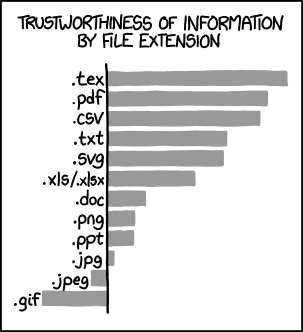
\includegraphics[width=.9\textwidth]{xkcd-fileextensions}~
          \rotatebox{90}{\tiny http://xkcd.com/1301 (CC-BY-NC 2.5)}
        }
      \end{column}
    } % End of \only<2->
  \end{columns}
\end{frame}

\begin{frame}
  \frametitle{Agenda}
  \tableofcontents
\end{frame}

\section{Einf\"uhrung}

\subsection{The Name of the Game}

\begin{frame}
  \frametitle{The Name of the Game}
  \framesubtitle{Just drop a view names}
  \begin{itemize}
  \item \TeX
    \begin{itemize}
    \item Donald E. Knuth, 1978
    \item Aktuell \TeX{} 3.1415926 (März~2008)
    \item Textsatzsystem mit eingebauter\\
      Makrosprache
    \item \enquote{The \TeX{}book}
    \end{itemize}
  \item \LaTeX
    \begin{itemize}
    \item Leslie Lamport, Anfang 1980er
    \item Aktuell \hologo{LaTeX2e}
    \item Makropaket für \TeX
    \item Meistverwendetste \TeX-Variante
    \item Unzählige Literatur
    \end{itemize}
  \item CTAN (Comprehensive \TeX{} Archive Network)
    \begin{itemize}
    \item über 4\,600 Pakete
    \item \texttt{CTAN://<pkg>} für \href{http://ctan.org}{\texttt{http://ctan.org/<pkg>}}
    \end{itemize}
  \end{itemize}
  \begin{textblock}{3}(0.72,0.17)
    \href{https://en.wikipedia.org/wiki/File:KnuthAtOpenContentAlliance.jpg}{%
      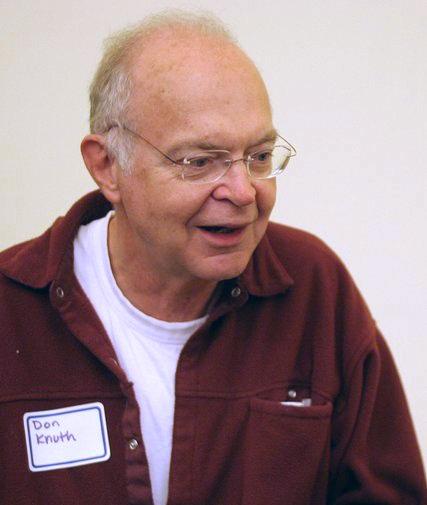
\includegraphics[width=3cm]{don-knuth}~%
      \rotatebox{90}{\tiny by Jacob Applebaum (CC-BY-SA 2.5)}%
    }
  \end{textblock}
  \begin{textblock}{3}(0.72,0.54)
    \href{https://en.wikipedia.org/wiki/File:Leslie_Lamport.jpg}{%
      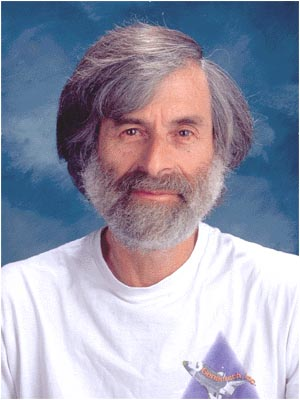
\includegraphics[width=3cm]{leslie-lamport}~%
      \rotatebox{90}{\tiny by Leslie Lamport}%
    }
  \end{textblock}
\end{frame}

\begin{frame}
  \frametitle{The Name of the Game (2)}
  \framesubtitle{Engines}
  \begin{itemize}
  \item \TeX\\
    7\,bit-ASCII, dvi-Ausgabe, v3.1415926
  \item pdf\TeX\\
    8\,bit-ASCII, dvi- oder pdf-Ausgabe, v1.40.14
  \item \hologo{XeTeX}\\
    UTF-8, Systemfonts (TTF, OTF), nur pdf-Ausgabe, schleppende
    Entwicklung, v0.9999.3
  \item \hologo{LuaTeX}\\
    UTF-8, Systemfonts (TTF, OTF), dvi- oder pdf-Ausgabe, Lua
    eingebettet, Arabischer Textsatz, v0.76
  \end{itemize}
\end{frame}

\subsection{Einf\"uhrungen}

\begin{frame}
  \frametitle{Einführungen}
  \nocite{*}
  \begingroup
  \printbibliography[heading=none,keyword=intro]
  \endgroup
\end{frame}

\subsection{\TeX-Distributionen}

\begin{frame}
  \frametitle{\TeX-Distributionen}
  \begin{itemize}
  \item \href{http://miktex.org}{\hologo{MiKTeX}} – nur für M\$
  \item \href{http://tug.org/texlive}{\TeX{} Live} – für Linux, M\$ \&
    Mac (Mac\TeX)
    \begin{itemize}
    \item M\$ über Installer
    \item Linux meist im Paketmanager
    \item \alert{aber} oft veraltet\dots
    \item Empfehlung: Immer \enquote{Vanilla \TeX{} Live}
      installieren!
    \item Apfel: Keine Ahnung
    \end{itemize}
  \item diverse weitere (oft veraltet)
  \item Apps für Android und iPad
  \end{itemize}
\end{frame}

\section{(Kryptische) Fehlermeldungen}

\subsection{Übliche Fehler}

\begin{frame}
  \frametitle{Tippfehler}
  \only<1->{%
    \begin{columns}[T]
      \begin{column}{.5\textwidth}
        \examplefile{examples/errors/typo.tex}
        \lstinputlisting[language={[LaTeX]TeX}]{examples/errors/typo.tex}
      \end{column}
      \begin{column}{.5\textwidth}
        Fehlermeldung:
        \lstinputlisting{examples/errors/typo.err}
      \end{column}
    \end{columns}
  }% End of \only<1->
  \only<2->{%
    \begin{itemize}
    \item Wahrscheinlich häufigster Fehler
    \item Tippfehler im Kommandonamen
    \item Kommando nicht definiert?
    \end{itemize}
    \begin{tikzpicture}[overlay]
      \draw[color=red,very thick] (2.85,3.3) circle (8pt);
    \end{tikzpicture}
  }
\end{frame}

\begin{frame}
  \frametitle{Überschreiben eines vorhandenen Kommandos}
    \begin{columns}[T]
      \only<1->{\begin{column}{.5\textwidth}
        \examplefile{examples/errors/renewcommand.tex}
        \lstinputlisting[language={[LaTeX]TeX}]{examples/errors/renewcommand.tex}
      \end{column}}
      \only<1>{\begin{column}{.5\textwidth}
        Fehlermeldung:
        \lstinputlisting{examples/errors/renewcommand.err}
      \end{column}}
      \only<2->{\begin{column}{.5\textwidth}
        Fehlermeldung:
        \lstinputlisting[lastline=3]{examples/errors/renewcommand.err}
        \end{column}}
    \end{columns}
  \only<2->{%
    \begin{itemize}
    \item Kommando schon definiert
    \item Überschreiben mit \texttt{\textbackslash renewcommand}\\
      \alert{Vorsicht!} Nur wenn man wirklich weiß, was man tut!
    \end{itemize}
    \begin{tikzpicture}[overlay]
      \draw[color=red,very thick] (0,4.35) circle (8pt);
    \end{tikzpicture}
  }
\end{frame}

\subsection{Mathemodus}

\begin{frame}[fragile]
  \frametitle{Zeichen mit besonderer Bedeutung}
  \only<1->{%
  \begin{columns}[T]
    \begin{column}{.5\textwidth}
      \examplefile{examples/errors/underscore.tex}
      \lstinputlisting[language={[LaTeX]TeX}]{examples/errors/underscore.tex}
    \end{column}
    \begin{column}{.5\textwidth}
      Fehlermeldung:
      \lstinputlisting{examples/errors/underscore.err}
    \end{column}
  \end{columns}
  }% End of \only<1->
  \only<2->{%
    \begin{itemize}
    \item Fehler wegen \texttt{\color{red}\_}
    \item Startet automatisch Mathemodus\\
      $\Rightarrow$ fehlendes \texttt{\$} am Ende
    \item Lösung: \texttt{\color{red}\textbackslash\_} 
    \end{itemize}
    \begin{tikzpicture}[overlay]
      \draw[color=red,very thick] (3.9,4.5) circle (8pt);
    \end{tikzpicture}
  }% End of \only<2->
\end{frame}

\begin{frame}[fragile]
  \frametitle{Klammerchaos}
  \only<1->{%
    \begin{columns}[T]
      \begin{column}{.5\textwidth}
        \examplefile{examples/errors/leftright.tex}
        \lstinputlisting[language={[LaTeX]TeX}]{examples/errors/leftright.tex}
      \end{column}
      \begin{column}{.5\textwidth}
        Fehlermeldung:
        \lstinputlisting{examples/errors/leftright.err}
      \end{column}
    \end{columns}
  }% End of \only<1->
  \only<2->{%
    \begin{itemize}
    \item Fehlendes \texttt{\color{red}\textbackslash right}
    \item Öffnend und schließend muss vorhanden sein
    \item \texttt{\color{red}\textbackslash right.} zur Unterdrückung
      der Klammer
    \item natürlich auch mit \texttt{\textbackslash left}\dots
    \end{itemize}
    \begin{tikzpicture}[overlay]
      \draw[color=red,very thick] (3.1,4.25) circle (8pt);
    \end{tikzpicture}
  }% End of \only<2->
\end{frame}

\begin{frame}[fragile]
  \frametitle{Klammerchaos (2)}
  \only<1->{%
    \begin{columns}[T]
      \begin{column}{.5\textwidth}
        \examplefile{examples/errors/brackets.tex}
        \lstinputlisting[language={[LaTeX]TeX}]{examples/errors/brackets.tex}
      \end{column}
      \begin{column}{.5\textwidth}
        Fehlermeldung:
        \lstinputlisting{examples/errors/brackets.err}
      \end{column}
    \end{columns}
  }% End of \only<1->
  \only<2->{%
    \begin{itemize}
    \item \texttt{\color{red}\}} schließt Gruppierung
    \item Escapen nötig: \texttt{\color{red}\textbackslash\}}
    \item \TeX{} kann genauen Fehler nicht feststellen\dots
    \end{itemize}
    \begin{tikzpicture}[overlay]
      \draw[color=red,very thick] (4.25,3.65) circle (8pt);
    \end{tikzpicture}
  }% End of \only<2->
\end{frame}

\begin{frame}
  \frametitle{Klammerchaos (3) – \texttt{align} sei Dank}
  \only<1>{%
  \examplefile{examples/errors/align.tex}
  \lstinputlisting[language={[LaTeX]TeX}]{examples/errors/align.tex}
  \begin{itemize}
  \item Gleicher Fehler wie eben (Zeile 5)
  \item \alert{aber\dots}
  \end{itemize}
  }% End of \only<1>
  \only<2>{%
    Die Fehlermeldung:
    \lstinputlisting[firstline=1,lastline=16]{examples/errors/align.err}
  }% End of \only<2>
  \only<3>{%
    \lstinputlisting[firstline=17,lastline=33,firstnumber=17]{examples/errors/align.err}
  }
  \only<4>{%
    \lstinputlisting[firstline=34,lastline=50,firstnumber=34]{examples/errors/align.err}
  }
  \only<5>{%
    \lstinputlisting[firstline=51,lastline=67,firstnumber=51]{examples/errors/align.err}
  }
  \only<6>{%
    \lstinputlisting[firstline=68,lastline=84,firstnumber=68]{examples/errors/align.err}
  }
  \only<7>{%
    \lstinputlisting[firstline=85,lastline=98,firstnumber=85]{examples/errors/align.err}
  }
  \only<8>)
  \item Übersicht im \LaTeX{} Companion
  \item Weitere Hilfe
    \begin{itemize}
    \item Internet-Recherche
    \item Mailinglisten (texhax, TEX-D-L)
    \item \href{http://tex.stackexchange.com}{TEX.sx}
    \end{itemize}
  \end{itemize}
\end{frame}

%%% Local Variables: 
%%% mode: latex
%%% coding: utf-8
%%% TeX-engine: luatex
%%% TeX-PDF-mode: t
%%% TeX-master: "../pr-ieee-main"
%%% End: 

\section{Grafiken}

\subsection{Grafiken einbinden}

\begin{frame}
  \frametitle{Grafiken einbinden}
  \begin{itemize}
  \item Viele Möglichkeiten, oft nicht trivial
  \item hier Übersicht, weiteres liefert Paketdokumentation
  \item Häufig verwendete Pakete:
    \begin{itemize}
    \item \texttt{graphicx}\\
      \emph{Der} Standard, eigentlich immer nötig
    \item \texttt{subfig}\\
      Möglichkeit Abbildungen zu gruppieren
    \item \texttt{wrapfig}\\
      Bilder im Fließtext
    \end{itemize}
  \end{itemize}
\end{frame}

\begin{frame}[fragile]
  \frametitle{\texttt{graphicx}}
  \framesubtitle{Grundlagen}
  \begin{itemize}
  \item Einbinden \texttt{\textbackslash usepackage\{graphicx\}}
  \item Zentraler Befehl \texttt{\textbackslash
      includegraphics[options]\{filename\}}
  \item Mögliche Werte für \texttt{options}:\\
    \texttt{width}, \texttt{height}, \texttt{angle}\dots
  \item Normales Einbinden:
\begin{lstlisting}[language={[LaTeX]TeX}]
\begin{figure}[ht]
  \centering
  \includegraphics[options]{filename}
  \caption{Caption text}
  \label{img:num}
\end{figure}
\end{lstlisting}
  \end{itemize}
\end{frame}

\begin{frame}
  \frametitle{\texttt{graphicx}}
  \framesubtitle{Gleitumgebungen}
  \begin{itemize}
  \item \texttt{figure} sog. Gleitumgebung
  \item wird von \TeX{} positioniert
  \item Positionierungswunsch
    \begin{itemize}
    \item \texttt{h}: here
    \item \texttt{t}: top
    \item \texttt{b}: bottom
    \item \texttt{p}: special page
    \end{itemize}
  \end{itemize}
\end{frame}

\begin{frame}
  \frametitle{\texttt{graphicx}}
  \framesubtitle{Weitere nützliche Befehle}
  \begin{itemize}
  \item \texttt{\textbackslash rotatebox\{angle\}\{text\}}\\
    Rotiert \texttt{text} um Winkel \texttt{angle}
  \item \texttt{\textbackslash
      scalebox\{h-scale\}\{v-scale\}\{text\}}\\
    Bietet die Möglichkeit, den \texttt{text} zu skalieren
  \item \texttt{\textbackslash reflectbox\{text\}}\\
    Spiegelt \texttt{text}
  \end{itemize}
\end{frame}

\begin{frame}
  \frametitle{\texttt{graphicx}}
  \framesubtitle{Beispiel}
  \examplefile{examples/graphics/graphic.tex}
  \fbox{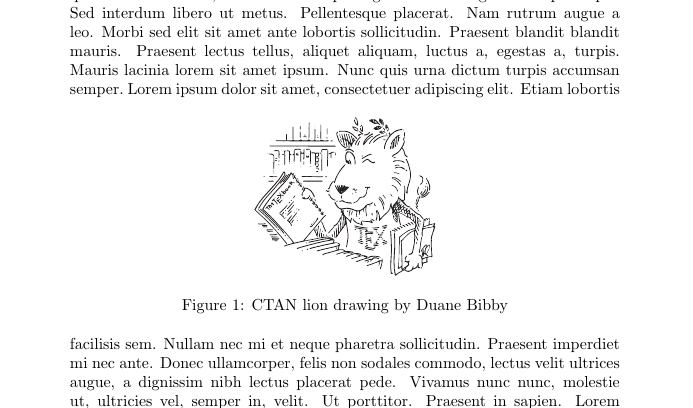
\includegraphics[width=.9\textwidth]{scr-graphic}}
\end{frame}

\begin{frame}
  \frametitle{\texttt{subfig}}
  
\end{frame}

\begin{frame}[fragile]
  \frametitle{\texttt{wrapfig}}
  \begin{itemize}
  \item Grundsätzlicher Code
\begin{lstlisting}[language={[LaTeX]TeX}]
\begin{wrapfigure}[lines]{placement}[overhang]{width}
  <figure>
\end{wrapfigure}
\end{lstlisting}
  \item Seltsame Effekte beim Seitenumbruch
  \item Empfehlung: Verzichten!
  \end{itemize}
\end{frame}

\begin{frame}
  \frametitle{\texttt{wrapfig}}
  \framesubtitle{Beispiel}
  \examplefile{examples/graphics/wrapfigure.tex}
  \fbox{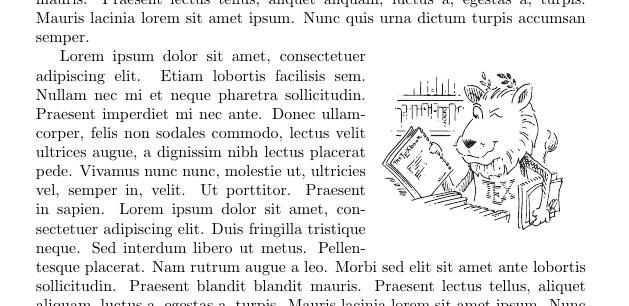
\includegraphics[width=.9\textwidth]{scr-wrapfigure}}
\end{frame}

\subsection{Grafiken erstellen}
\begin{frame}
  \frametitle{Grafiken erstellen}
  Mehrere Möglichkeiten
  \begin{itemize}
  \item \hologo{METAPOST}\\
    basiert auf \hologo{METAFONT}
  \item PSTricks\\
    verwendet PostScript für die Graphikerstellung
  \item Ti\emph{k}Z\\
    komplett \TeX-basierend
  \end{itemize}
\end{frame}

\begin{frame}[fragile]
  \frametitle{\hologo{METAPOST}}
  \begin{columns}[T]
    \begin{column}{.25\textwidth}
      \begin{mplibcode}
beginfig(1);
    numeric u; u=50pt;
    pickup pencircle scaled 2pt;
    draw fullcircle scaled 1u;
    draw (-.3u,-.1u)..(0,-.3u)..(.3u,-.1u);
    pickup pencircle scaled 4pt;
    draw (0,0);
    pickup pencircle scaled 7pt;
    draw (-.2u,.2u); draw (.2u,.2u);
endfig;
      \end{mplibcode}
    \end{column}
    \begin{column}{.75\textwidth}
      \examplefile{examples/graphics/smiley.mp}
      \lstinputlisting[language=MetaPost]{examples/graphics/smiley.mp}
    \end{column}
  \end{columns}
\end{frame}

\begin{frame}
  \frametitle{\hologo{METAPOST} (2)}
  \begin{itemize}
  \item Vorträge von DANTE2013 für Einsteiger:
    \begin{itemize}
    \item
      \href{http://www.dante.de/events/dante2013/Programm/Vortraege/folien-entenmann.pdf}{Walter
      Entenmann – Graphik mit \hologo{METAPOST}}
    \item
      \href{http://www.dante.de/events/dante2013/Programm/Vortraege/folien-voipio.pdf}{Mari
      Voipio – Entry-Level MetaPost}
    \end{itemize}
    \item Übersetzung mit \texttt{mpost smiley.mp}\\
    $\rightarrow$ \texttt{smiley.1} (ähnlich EPS-Graphik)
  \item Einbinden mit \texttt{\textbackslash includegraphics}\\
    Kein \hologo{pdfLaTeX}!  Umweg über PostScript notwendig
  \item Direkte Verwendung mit \hologo{LuaTeX} (\texttt{\href{http://ctan.org/pkg/luamplib}{CTAN://pkg/luamplib}})
  \end{itemize}
\end{frame}

\begin{frame}
  \frametitle{PSTricks}
  \begin{columns}[T]
    \begin{column}{.25\textwidth}
      
\includegraphics[width=2cm]{smiley-pstricks}
    \end{column}
    \begin{column}{.75\textwidth}
      \examplefile{examples/graphics/smiley-pstricks.tex}
      \lstinputlisting[language={[LaTeX]TeX}]{examples/graphics/smiley-pstricks.tex}
    \end{column}
  \end{columns}
\end{frame}

\begin{frame}
  \frametitle{PSTricks (2)}
  \begin{itemize}
  \item Übersetzung (um PDF zu erhalten) mit\\
    \texttt{\$ latex smiley-pstricks.tex}\\
    \texttt{\$ dvips smiley-pstricks.dvi}\\
    \texttt{\$ ps2pdf smiley-pstricks.ps}
  \item Funktioniert \emph{nicht} mit \hologo{LuaTeX}, nur
    \hologo{LaTeX} und \hologo{XeTeX}
  \item Über 100~Pakete auf CTAN
  \item Galerie auf \href{http://pstricks.tug.org}{pstricks.tug.org}
  \end{itemize}
  \begingroup
  \printbibliography[heading=none,keyword=graphic]
  \endgroup
\end{frame}

\begin{frame}
  \frametitle{Ti\emph{k}Z}
  \begin{columns}[T]
    \begin{column}{.25\textwidth}
      
\includegraphics[width=2cm]{smiley-tikz}
    \end{column}
    \begin{column}{.75\textwidth}
      \examplefile{examples/graphics/smiley-tikz.tex}
      \lstinputlisting[language={[LaTeX]TeX}]{examples/graphics/smiley-tikz.tex}
    \end{column}
  \end{columns}
\end{frame}

\begin{frame}
  \frametitle{Ti\emph{k}Z (2)}
  \begin{itemize}
  \item Kein Buch, nur PDF-Dokumentation (726 Seiten)
  \item Funktioniert mit allen \TeX-Interpretern
  \item Funktionsumfang ähnlich PSTricks
  \item Galerie auf \href{http://www.texample.net}{texample.net}
  \item Diversen Erweiterungspakete
  \item Viele Beispiele auch auf \href{http://tex.stackexchange.com}{\TeX.sx}
  \end{itemize}
\end{frame}

%%% Local Variables: 
%%% mode: latex
%%% coding: utf-8
%%% TeX-engine: luatex
%%% TeX-PDF-mode: t
%%% TeX-master: "../pr-ieee-main"
%%% End: 

% Graphiken
% Präsentationen

\begin{frame}
  \frametitle{Fazit}
  \begin{itemize}
  \item \hologo{(La)TeX} als Tool für alles (möglich)
  \item Zum Teil hoher Lernaufwand\\
    \begin{itemize}
    \item Am Besten sofort anfangen
    \item \LaTeX{} z.\,B. während SEP lernen\\
      fast unmöglich
    \item Wie Programmieren, lernen nur\\
      durch selbst machen
    \end{itemize}
  \item Bücher, Dokumentationen,\\
    Internetseiten, Mailinglisten
  \item (Zeitaufwändiges) Hobby {\Huge ☺}
  \end{itemize}
  \begin{textblock}{5.5}(0.57,0.47)
    
\includegraphics[width=5cm]{lion}~
    \rotatebox{90}{\tiny CTAN lion draw­ing by Duane Bibby}
  \end{textblock}
\end{frame}

{\usebackgroundtemplate{%
  \tikz\node[opacity=0.3]{%
    
\includegraphics[width=\paperwidth,height=\paperheight]{tex-background}%
  };%
}
\begin{frame}
  \frametitle{The End\dots}
  \begin{textblock}{10}(0.3,0.4)
    {\Huge\color{red}Happy \TeX-ing!}
  \end{textblock}
  \begin{textblock}{10}(0.1,0.88)
    \small All files available at
    \href{https://github.com/sl-gap/tex-tutorial/}{https://github.com/sl-gap/tex-tutorial/}
  \end{textblock}
\end{frame}
}

\end{document}

%%% Local Variables: 
%%% mode: latex
%%% coding: utf-8
%%% TeX-engine: luatex
%%% TeX-PDF-mode: t
%%% TeX-master: t
%%% End: 
